\documentclass[11pt,a4paper]{article}

\usepackage[a4paper, top=2.5cm, bottom=2.5cm, left=2.5cm, right=2.5cm]{geometry}
\usepackage{fancyhdr}
\usepackage{booktabs}
\usepackage{array}
\usepackage{tabularx}
\usepackage{tikz}
\usetikzlibrary{calc, positioning, arrows.meta, shapes, fit, backgrounds}
\usepackage{eso-pic}
\usepackage{enumitem}
\usepackage{caption}
\usepackage{textcomp}
\usepackage{microtype}
\usepackage{hyperref}
\usepackage{xcolor}
\usepackage{listings}
\usepackage{amsmath}

\hypersetup{colorlinks=false,pdfborder={0 0 0}}

% Page frame on every page (drawn behind content)
\AddToShipoutPictureBG{%
  \begin{tikzpicture}[remember picture, overlay]
    \draw[line width=0.4pt]
      ([xshift=1.25cm, yshift=1.35cm]current page.south west)
      rectangle
      ([xshift=-1.25cm, yshift=-0.85cm]current page.north east);
  \end{tikzpicture}%
}

% Headers
\pagestyle{fancy}
\fancyhf{}
\fancyhead[L]{\small TruthOracle Prediction Market Protocol}
\fancyhead[R]{\small Draft}
\fancyfoot[C]{\thepage}
\renewcommand{\headrulewidth}{0.4pt}
\renewcommand{\footrulewidth}{0pt}

% Daml listings
\lstdefinelanguage{daml}{
  morekeywords={module, where, import, template, with, signatory, observer,
    controller, do, choice, agreement, returns, key, maintainer, let, in,
    if, then, else, data, deriving, interface, viewtype, type, instance, this,
    create, exercise, fetch, archive, abort, assertMsg, assert, getTime, Update,
    Party, Text, Int, Decimal, ContractId, Bool, Optional, Some, None, True, False,
    pure, ensure, postconsuming, nonconsuming, case, of, elem, Time, mapA, foldl,
    length, filter, all, forA, any, sha256, secp256k1},
  sensitive=true,
  morecomment=[l]{--},
  morecomment=[s]{\{-}{-\}},
  morestring=[b]"
}

\lstset{
  basicstyle=\footnotesize\ttfamily,
  keywordstyle=\bfseries,
  showstringspaces=false,
  frame=single,
  framesep=5pt,
  framerule=0.4pt,
  language=daml,
  breaklines=true,
  columns=fullflexible,
  aboveskip=8pt,
  belowskip=8pt
}

\setlength{\parindent}{1.5em}
\setlength{\parskip}{0.4em}

\begin{document}

% ---- TITLE PAGE ----
\thispagestyle{empty}
\vspace*{2cm}

\begin{center}
{\scshape Technical Proposal}\\[3pt]
{\footnotesize\scshape Canton Application Layer\ \ $\vert$\ \ Prediction Markets}
\end{center}

\vspace{1.5cm}
\noindent\rule{\linewidth}{0.4pt}

\vspace{0.5cm}
\begin{center}
{\Large\bfseries TruthOracle: A Canton-Native Prediction Market\\ with pm-AMM and Tiered Objective Resolution\par}
\end{center}

\vspace{0.4cm}
\noindent\rule{\linewidth}{0.4pt}

\vspace{1.5cm}
\begin{center}
\itshape
A privacy-preserving prediction market protocol with dynamic pm-AMM liquidity\\
and deterministic, source-grounded resolution from named, accountable data sources.\\
No UMA / Pyth oracle dependency. Built on Canton.
\end{center}

\vspace{2cm}
\begin{center}
\begin{tabular}{r l}
\textbf{Author:} & Sachin Jangid \\[6pt]
\textbf{Status:}  & Draft \\
\textbf{Version:} & 0.7 \\
\textbf{Requires:} & CIP-56 (token semantics) \\
\textbf{License:} & Apache-2.0 \\[6pt]
\textbf{Created:} & 18 February 2026 \\
\textbf{Revised:} & 22 July 2026 \\
\end{tabular}
\end{center}
\vfill

\newpage

% ---- ABSTRACT ----
\section{Abstract}

This proposal defines TruthOracle, a Canton-native prediction market protocol composed of four Daml primitives: a \textbf{Market} contract holding a \emph{dynamic} prediction-market automated market maker (pm-AMM, Gaussian score dynamics) over binary outcome shares; typed \textbf{Position} contracts representing outcome holdings owned by traders; an \textbf{Outcome Attestation} contract carrying a signed claim about what an allowlisted data source reported; and a \textbf{Liquidity Position} contract representing pro-rata claims on the pm-AMM reserve. A fifth, optional family of contracts --- the \textbf{Prediction Model} marketplace --- lets external forecasters commit timestamped predictions and earn from a fee-funded prize pool when they beat the market. Off-ledger services --- a read model over the Participant Query Store for dashboards and audit reporting, and an operator console with source/reporter key custody --- orchestrate presentation and signing but hold no authority the ledger does not grant.

Resolution is \emph{deterministic} and \emph{objective}. TruthOracle adopts a \textbf{tiered resolution model} drawn from how production prediction markets and oracle networks already work, adapted to Canton's identity-bearing, privacy-preserving ledger: (T0) a designated licensed operator records the result (the Kalshi model); (T1) the authoritative source signs its data and the Market verifies an ordinary digital signature on-ledger using Daml's \texttt{DA.Crypto.Text} primitives (the Pyth / API3 first-party-oracle model); (T2) a quorum of independent, allowlisted reporters each fetch the source and submit signed attestations that must agree (the Chainlink aggregation model); and (T3) an optional optimistic propose-and-challenge layer with collateral bonds (the Polymarket UX), whose disputes escalate \emph{objectively} to T1/T2 rather than to token-holder voting. Every tier reduces to ordinary signatures, hashes, and Daml authorization. The protocol does not depend on UMA, Pyth, or any external oracle, inherits Canton's sub-transaction privacy, and is implementable today on Canton DevNet with no changes to the Canton protocol or synchronization domain software.

% ---- MOTIVATION ----
\section{Motivation}

Public-chain prediction markets face three structural problems that limit their use beyond a small set of high-attention events. These mirror the three problems set out in the TruthOracle pitch: order-book/matching frictions, oracle resolution risk, and an engagement deficit.

\textbf{Thin order books.} Centralized limit order book designs (Polymarket, Kalshi) require a counterparty to be present at the same price level at the same time. Outside top markets, book depth collapses, slippage becomes prohibitive at small ticket sizes, and market makers cannot economically service tail markets. Automated market makers, well-studied in the spot trading context, have not yet seen wide deployment in prediction markets, in part because spot AMMs (e.g., constant product) do not naturally bound prices to the $[0, 1]$ probability simplex.

\textbf{Resolution by intersubjective oracle.} Polymarket and similar venues resolve through UMA's Optimistic Oracle. The Optimistic Oracle resolves correctly under normal conditions but degrades under disputes: bonds are large, resolution can be delayed by 48 hours or longer, and several high-value markets have resolved against the source factual answer in cases where token holders had aligned positions. Practitioners increasingly distinguish between \emph{intersubjective resolution} (what a quorum of token holders agrees happened) and \emph{objective resolution} (what an authoritative source reports). Licensed gaming operators cannot accept the former.

\textbf{Engagement deficit.} The most knowledgeable participants in any prediction domain --- sports analysts, electoral statisticians, on-chain data scientists --- frequently do not participate as traders. Their forecasts are published as static graphics on social platforms; the information is incorporated into market prices only when traders manually translate it. The result is a market structure in which expertise is observed but not priced.

Canton already provides the trust and coordination primitives that solve adjacent problems in capital markets: sub-transaction privacy, multi-party atomic composition, and Daml-mediated authorization. This proposal extends those primitives to prediction markets. The key value additions of the protocol are:

\begin{itemize}[leftmargin=2em, itemsep=2pt]
  \item \textbf{Constant liquidity via a dynamic pm-AMM.} A pm-AMM pool prices both outcomes simultaneously from the normal CDF, so any trade size receives a quote without waiting for a counterparty; its liquidity decays toward expiry, holding LP risk (loss-versus-rebalancing) uniform and predictable.
  \item \textbf{Deterministic, objective resolution.} A tiered model (\S\ref{sec:resolution}) settles markets from named, accountable sources using ordinary signatures and Daml authorization, avoiding the intersubjective dispute window of UMA-style oracles entirely.
  \item \textbf{Trust from identity and accountability.} Because Canton parties are real, licensed, and auditable, a source's or reporter's signature \emph{is} the guarantee of provenance, enforced by Daml's authorization model.
  \item \textbf{Privacy-preserving by default.} Position sizes, trade prices, and trader identities are visible only to the parties involved and explicitly designated audit observers, inheriting Canton's stakeholder-projection model.
  \item \textbf{Expertise that is priced, not just observed.} An optional Prediction Model marketplace lets forecasters commit timestamped predictions on-ledger and earn from a fee-funded prize pool when they beat the market, turning the engagement deficit into a contribution loop.
  \item \textbf{Composable with existing Canton workflows.} The Market accepts any Canton-native fungible token as collateral and emits standard Daml events consumable by Cantor8 wallets, custodians, and compliance systems without bespoke integration.
\end{itemize}

Target use cases include sports markets resolved against licensed data feeds (Opta, Sportradar), electoral and policy markets resolved against state-published endpoints, financial-event markets resolved against exchange APIs, and brand-sponsored markets where the sponsor is the named audit observer.

% ---- HOW OTHERS RESOLVE ----
\section{How Existing Prediction Markets Resolve}
\label{sec:related}

Resolution is the hardest part of a prediction market: liquidity is an engineering problem, but resolution is a trust problem. Before specifying TruthOracle's design we survey how the field solves it today, because the tiered model in \S\ref{sec:resolution} is assembled deliberately from the parts of these designs that survive on a licensed, privacy-preserving ledger.

\begin{center}
\begin{tabular}{p{2.6cm} p{5.2cm} p{5.6cm}}
\toprule
\textbf{Venue} & \textbf{Mechanism} & \textbf{Trust basis / limitation} \\
\midrule
Polymarket (UMA Optimistic Oracle) & A proposer posts an outcome with a bond; if unchallenged in a window it stands, else UMA token holders vote. & \emph{Intersubjective}: the answer is what a token quorum says, which can diverge from fact when voters hold positions. Slow under dispute. \\[4pt]
Augur & Designated reporter posts, then escalating dispute rounds backed by REP staking. & Intersubjective and slower; forking is catastrophic-case only. \\[4pt]
Kalshi & A CFTC-licensed exchange settles from named authoritative sources. & \emph{Objective and fast}, but fully centralized; trust is the operator's license and legal accountability. \\[4pt]
Chainlink & $N$ independent node operators fetch a feed; the contract aggregates (median) on-chain; reputation and staking. & Objective; needs an operator network and an aggregation rule. \\[4pt]
Pyth / API3 & \emph{First-party} oracle: the data source itself signs its data; the signature is verified on-chain (API3 removes the middleman entirely). & Objective; trust is the source's own key. Requires the source to sign. \\
\bottomrule
\end{tabular}
\end{center}

Two lessons drive the TruthOracle design. First, \textbf{objective beats intersubjective} for a licensed venue: Kalshi, Chainlink, and Pyth all resolve to ``what an authoritative source reported,'' which is exactly what a regulator and a licensed operator require, whereas UMA/Augur resolve to ``what a token quorum decided.'' Second, \textbf{provenance is cheapest when the source vouches for its own data.} The first-party model (Pyth/API3) lets the authoritative source sign the data it publishes, so an ordinary digital-signature check establishes where a value came from --- no intermediary need be trusted. On Canton this is the natural fit: every party is a real, licensed identity, and a signature on a contract, enforced by Daml's authorization model, is itself a provenance guarantee. TruthOracle therefore combines the objective-source spirit of Kalshi/Chainlink/Pyth with the open, optimistic UX of Polymarket, while excluding intersubjective token voting.

% ---- SPEC ----
\section{Specification and Implementation}

The protocol comprises four core contract types, summarised below, composing into a four-phase market lifecycle: creation, trading, resolution, and redemption. A fifth, optional contract family supports the Prediction Model marketplace (\S\ref{sec:models}). Each phase is initiated by a typed Daml choice; intermediate state is held in separate contracts so that authorization, privacy, and lifecycle observability can be reasoned about independently.

\vspace{0.4em}
\begin{center}
\begin{tabular}{p{4.5cm} p{9.5cm}}
\toprule
\textbf{Contract} & \textbf{Role} \\
\midrule
Market & Holds market metadata, the pm-AMM reserve state, the resolution policy (allowlisted sources, source public keys, reporter set, quorum, and which tiers are enabled). \\
Position & Represents a trader's holding of YES or NO outcome shares, signed by the trader. \\
Liquidity Position & Represents an LP's share of the pm-AMM reserve, redeemable for proportional collateral plus accrued fees. \\
Outcome Attestation & Carries a signed claim --- from the source itself, from a reporter, or from a proposer --- about what the allowlisted source returned, plus the asserted outcome. Created only after market expiry. \\
\bottomrule
\end{tabular}
\end{center}

\subsection{Market Contract}

The Market is the central primitive. An operator (a participant authorized by the platform, typically a Cantor8-licensed subsidiary) creates a Market to make a binary prediction tradeable. The Market signatories are the operator and the platform treasury; traders interact through observer-controlled choices.

\vspace{0.3em}
\begin{center}
\begin{tabular}{p{3.7cm} p{10.3cm}}
\toprule
\textbf{Field} & \textbf{Purpose} \\
\midrule
Operator & Signatory; the market-making entity. \\
Treasury & Signatory; on-ledger custodian of pooled collateral. \\
Market Id & Globally unique handle within the operator's scope. \\
Question & Human-readable market question (UTF-8, $\leq 256$ characters). \\
Resolution Policy & The tiered policy of \S\ref{sec:resolution}: enabled tiers, the source allowlist, each source's pinned public key (for T1), the reporter allowlist and quorum (for T2), and the challenge window and bond size (for T3). Immutable after creation. \\
Liquidity Period & Optional pre-trading liquidity-collection window (dynamic pools): swaps are disabled until it elapses, while complete-set minting and liquidity provision are open; it is also the anchor from which effective liquidity decays. \\
Expiry & Timestamp after which trading stops and resolution becomes enabled. \\
Grace Period & Duration after expiry within which resolution must complete; otherwise the market voids. \\
Collateral Token & Canton-native fungible token used to fund and pay out positions. \\
Reserve YES / NO ($x$, $y$) & Decimal share counts of the pm-AMM's YES and NO inventory. \\
Liquidity Param $L$ & Scales pm-AMM pool depth; effective liquidity decays as $L\sqrt{T-t}$ toward Expiry (dynamic pm-AMM). \\
Fee Bps & Per-trade fee, in basis points, taken from the input side. \\
Status & Trading, Expired, Proposed, Resolved, or Voided. \\
Audit Observers & Read-only parties (compliance officers, licensed sponsors). \\
\bottomrule
\end{tabular}
\end{center}

The Market exposes these classes of choices, each enforcing its own preconditions:

\begin{itemize}[leftmargin=2em, itemsep=2pt]
\item \texttt{ProvideLiquidity} (any observer, before expiry) --- deposits collateral and mints a Liquidity Position; open during the liquidity period.
\item \texttt{Buy} / \texttt{Sell} (any observer, after the liquidity period, before expiry) --- the collateral-denominated pm-AMM trading surface; creates or consumes Position contracts.
\item \texttt{SwapShares} (any observer, after the liquidity period, before expiry) --- the direct outcome-token swap (deposit YES receive NO, or vice versa), the primitive trading operation of the reference pm-AMM implementation; \texttt{Buy}/\texttt{Sell} compose it with complete-set minting/merging for one-step collateral trades.
\item \texttt{Split} / \texttt{Merge} (any observer, before expiry) --- mint or burn \emph{complete sets}: one unit of collateral mints one YES plus one NO share (and conversely), the no-arbitrage peg that keeps the system fully collateralized.
\item \texttt{Resolve} (operator, after expiry) --- settles the Market via the enabled resolution tier(s) of \S\ref{sec:resolution}.
\item \texttt{ProposeOutcome} / \texttt{Challenge} / \texttt{Finalize} (T3 only) --- the optional optimistic flow.
\item \texttt{Void} (operator, after expiry + grace period) --- transitions to Voided when no tier produced a valid resolution.
\end{itemize}

\subsection{Dynamic pm-AMM Pool (Gaussian Score Dynamics)}

The Market holds the pm-AMM reserves as inline fields. Reserves $(x, y)$ represent shares of YES and NO outstanding in the pool, and a liquidity parameter $L$ scales pool depth. TruthOracle adopts \href{https://www.paradigm.xyz/2024/11/pm-amm}{Paradigm's prediction-market AMM}, in which price is the cumulative normal distribution of a Brownian ``score'' rather than a ratio of reserves, so a quote is a calibrated probability that always lies on the $[0,1]$ simplex. The marginal price of the YES share is
\[
P_{\mathrm{YES}} = \Phi\!\left(\frac{y - x}{L_{\mathrm{eff}}}\right), \qquad P_{\mathrm{NO}} = 1 - P_{\mathrm{YES}},
\]
where $\Phi$ is the standard normal CDF; because $\Phi \in [0,1]$, reserves can never quote outside the simplex.

The pool is \emph{dynamic}: effective liquidity decays toward expiry as $L_{\mathrm{eff}} = L\sqrt{T - t}$ (with $T$ the market Expiry and $t$ the current time), and trades satisfy the time-dependent invariant
\[
(y - x)\,\Phi(z) + L_{\mathrm{eff}}\,\phi(z) - y = 0, \qquad z = \frac{y - x}{L_{\mathrm{eff}}},
\]
with $\phi$ the normal PDF. As $t \to T$ liquidity is systematically withdrawn, holding the expected loss-versus-rebalancing to a constant fraction of pool value --- a \emph{uniform} AMM whose instantaneous $\mathrm{LVR}_t = V_t / 2(T - t)$ integrates to a predictable total of $\approx V_0/2$ over the market's life, so liquidity provision is a calculable business rather than the guaranteed loss-at-expiry of a constant-product curve. Liquidity is added \emph{by value}: an LP names a desired value increase $\Delta V(P)$, and the pool derives the liquidity change $\Delta L = \Delta V(P) / \phi(\Phi^{-1}(P))$ and the exact YES/NO deposits that leave the current price unchanged.

Both the optimal reserves and the deposit sizing are \emph{closed-form} in the price: at price $P$ the pool holds
\[
x^*(P) = L\bigl(\Phi^{-1}(P)\,P + \phi(\Phi^{-1}(P)) - \Phi^{-1}(P)\bigr), \qquad
y^*(P) = L\bigl(\Phi^{-1}(P)\,P + \phi(\Phi^{-1}(P))\bigr),
\]
so $y^*(P) - x^*(P) = L\,\Phi^{-1}(P)$ and $V(P) = L\,\phi(\Phi^{-1}(P))$. Liquidity provision and reserve sizing therefore need no root-finding; only a swap --- price given a trade size --- requires a one-dimensional solve of the invariant.

A per-trade fee of $\phi_{\mathrm{fee}}$ basis points is retained in the pool; liquidity providers earn it proportionally to their Liquidity Position share at redemption. The \texttt{Buy} choice validates the trader's slippage bound, solves the invariant for the new reserves, debits collateral, and creates a Position; execution is all-or-nothing.

\emph{Execution model (following the reference pm-AMM implementation).} The Market caches the current price and executes every trade against \emph{virtual reserves} --- the closed-form optimal reserves $x^*(P), y^*(P)$ for the cached price at the current effective liquidity --- while the physical reserve fields custody inventory for solvency accounting. This keeps the quoted price continuous under time-decaying $L_{\mathrm{eff}}$ (the price moves only when trades move it, not as a side-effect of decay). Collateral enters and leaves the system only through \emph{complete sets}: one unit of collateral mints one YES plus one NO share (\texttt{Split}) and conversely (\texttt{Merge}), so a \texttt{Buy} is a mint-and-swap and a \texttt{Sell} its inverse, and each winning share redeems for exactly one unit at settlement. Dynamic pools may open with a short pre-trading \emph{liquidity period} during which only liquidity provision and complete-set minting are enabled, letting LPs seed depth before price discovery begins; effective liquidity decays from the end of that window. The pm-AMM is pure Daml arithmetic over \texttt{Decimal}, realised by a small math library --- the normal-distribution functions $\Phi$, $\phi$, and $\Phi^{-1}$ via rational approximation, fixed-point helpers, and a one-dimensional solver for the swap-direction invariant (reserve and liquidity sizing are closed-form) --- and is wholly independent of the resolution mechanism.

\subsection{Outcome Share Tokens (Positions)}

A Position is a typed Daml contract representing a holder's YES or NO share holding for a single Market, signed by the holder, observed by the operator for accounting and by audit observers for compliance.

\vspace{0.3em}
\begin{center}
\begin{tabular}{p{3.5cm} p{10.5cm}}
\toprule
\textbf{Field} & \textbf{Role} \\
\midrule
Holder & Signatory; the trader who owns the shares. \\
Operator & Observer; required for pm-AMM accounting and audit projection. \\
Market Ref & Textual reference to the originating Market by identifier. \\
Outcome & \texttt{YES} or \texttt{NO}. \\
Shares & Decimal share count. \\
Cost Basis & Collateral originally paid; used for void refunds and tax accounting. \\
Audit Observers & Inherited from the Market for compliance visibility. \\
\bottomrule
\end{tabular}
\end{center}

Positions support three terminal choices: \texttt{Redeem} (holder, after resolution: one collateral unit per winning share, zero per losing share, cost basis if Voided), \texttt{SellBack} (holder, before resolution: returns shares to the pm-AMM for its quoted output collateral), and \texttt{Transfer} (holder: reassigns ownership). Positions are visible to the holder, the operator, and the audit observers only; the protocol exposes no aggregate-positions endpoint to non-audit parties.

% ---- RESOLUTION ----
\section{Objective Resolution}
\label{sec:resolution}

Resolution is a \textbf{tiered policy}, fixed at Market creation, in which each tier reduces to ordinary signatures, hashes, and Daml authorization. An operator enables one or more tiers per market according to the source's capabilities and the market's value. All four tiers settle to an objective outcome; none uses intersubjective voting.

\subsection{The Outcome Attestation}

Every tier produces or consumes a single shared contract, the \texttt{OutcomeAttestation}. Its signer and which optional fields are populated differ by tier, but the Market's \texttt{Resolve} logic treats them uniformly.

\vspace{0.3em}
\begin{center}
\begin{tabular}{p{3.3cm} p{10.7cm}}
\toprule
\textbf{Field} & \textbf{Role} \\
\midrule
Attester & Signatory; the party staking its identity on this reading (a source, a reporter, or a proposer). \\
Operator & Observer; will exercise \texttt{Resolve} / \texttt{Finalize}. \\
Market Ref & The Market being resolved. \\
Source Uri & The allowlisted source the reading came from. \\
Fetched At & Timestamp of the reading. \\
Outcome & \texttt{YES}, \texttt{NO}, or \texttt{Void}. \\
Payload Hash & \texttt{sha256} of the verbatim source response, committing the attester to a specific reading and enabling dispute reconstruction. \\
Source Signature & (T1 only) the source's own signature over the payload; \texttt{None} for reporter/proposer attestations. \\
Response Excerpt & Optional human-readable snippet (e.g., the final scoreline) retained for audit observers. \\
\bottomrule
\end{tabular}
\end{center}

\subsection{Tier 0 --- Designated Operator (Kalshi model)}

The simplest tier, and the one the current reference deployment uses: the licensed operator reads the result from the named source and records it directly through a \texttt{Resolve} that accepts an operator-signed attestation. Trust is the operator's license, legal accountability, and the immutable, audit-visible record of which source it named at creation. This tier is appropriate for low-value markets and for regulated venues where the operator is already the legally responsible settlement agent. It is fast and requires nothing of the source. Its weakness --- a single trusted party --- is precisely what tiers T1--T3 progressively remove.

\subsection{Tier 1 --- First-Party Signed Source (Pyth / API3 model)}

\begin{sloppypar}
When the authoritative source can sign its data --- directly, or via a data desk that re-publishes signed payloads --- TruthOracle uses its strongest tier. At Market creation the operator pins the source's public key in the Resolution Policy. To resolve, the source (or its data desk) produces a payload (the verbatim result), signs its \texttt{sha256} hash, and an \texttt{OutcomeAttestation} is created carrying the payload hash, the outcome, and the source signature. The Market's \texttt{Resolve} verifies the signature \emph{on-ledger} with \texttt{DA.Crypto.Text.secp256k1}, which checks a secp256k1 signature against a message hash and a public key --- ordinary public-key cryptography, the same family of primitive that underpins TLS itself. The check establishes exactly one fact: this byte string was signed by the holder of the pinned key. Trust therefore reduces to the source's own key, with no intermediary to vouch for the data. This is the API3 first-party-oracle pattern, expressed in Daml.
\end{sloppypar}

\subsection{Tier 2 --- Independent Reporter Quorum (Chainlink model)}

When the source cannot sign on-ledger (most public HTTPS endpoints today), TruthOracle falls back to redundancy across accountable parties. At creation the operator names a set of $N$ independent, allowlisted reporter parties and a quorum threshold $M$. After expiry each reporter independently fetches the allowlisted source over ordinary TLS, optionally using an AI/LLM parser to extract the outcome from a semi-structured page (the parser's output is ordinary data the reporter vouches for, not a proven computation), and creates a reporter-signed \texttt{OutcomeAttestation} carrying the payload hash and outcome. \texttt{Resolve} admits the resolution only when $M$ attestations, from distinct allowlisted reporters reading allowlisted sources within the window, agree on the same outcome. Trust is $M$-of-$N$ redundancy plus the reporters' reputation and off-ledger legal accountability --- the Chainlink aggregation idea, with named licensed parties instead of an anonymous node network. A single dishonest or mistaken reporter cannot move the result.

\subsection{Tier 3 --- Optimistic Propose-and-Challenge (Polymarket UX, objective escalation)}

\begin{sloppypar}
To preserve the open, anyone-can-resolve UX of Polymarket --- and the pitch's ``turbo-charged'' feel --- without inheriting UMA's intersubjective voting, TruthOracle offers an optional optimistic layer that escalates \emph{objectively}. A proposer posts an \texttt{OutcomeAttestation} and bonds collateral via \texttt{ProposeOutcome}; the Market enters \texttt{Proposed}. If the challenge window elapses with no challenge, anyone may \texttt{Finalize} and the proposed outcome stands (the fast, cheap happy path that covers the overwhelming majority of markets). If a challenger disagrees, it posts an opposing attestation and an equal bond via \texttt{Challenge}; this does \emph{not} trigger a token vote. Instead it escalates to an authoritative tier: T1 if the source can sign, otherwise the T2 reporter quorum. The authoritative outcome settles the market, the bond of the party who was wrong is slashed to the party who was right (deterring frivolous proposals and challenges symmetrically), and resolution still rests on an objective source rather than on a popularity contest. This gives Polymarket-style openness and speed with Kalshi-grade objectivity.
\end{sloppypar}

\subsection{Choosing tiers}

The tiers are complementary, not exclusive. A typical configuration: enable T3 for open participation and speed, with T2 as its escalation backstop, and T1 wherever the source offers signed data. Low-value or internal markets may run T0 alone. High-value markets should require T2 (or T1$+$T2) and a longer challenge window. Because the policy is immutable from creation and visible to audit observers, traders and regulators can see ex ante exactly how a given market will be resolved.

\subsection{Cryptographic basis}

\begin{sloppypar}
The protocol relies only on standard, well-understood cryptography, all of it available in the Daml standard library (\texttt{DA.Crypto.Text}). Two primitives appear. \texttt{sha256} commits an attestation to the verbatim source payload (the \texttt{payloadHash}), so any later reading can be checked byte-for-byte against what was attested and disputes can be reconstructed. \texttt{secp256k1} digital-signature verification confirms, in T1, that a signed payload came from the holder of a pinned source key. Beyond these, provenance rests on Daml's authorization model: the act of signing a contract already establishes which party produced it, so an attestation's signer field is self-authenticating. Because every relevant participant --- operator, source, reporter, proposer --- is a named, accountable, allowlisted Canton identity, these primitives together with the authorization model make resolution verifiable and auditable, and the trust they encode (a licensed operator, a signing source, a quorum of reputable reporters, bonded challengers) is exactly the trust a regulated venue is organised to supply.
\end{sloppypar}

\subsection{Daml Reference Templates}

The contract types are realised in a small Daml package (\texttt{daml/TruthOracle/} in the Cantor8 monorepo; SDK 3.x). Shared types are listed first, then the Market's resolution logic. The Position, Liquidity Position, and Outcome Attestation templates follow the same shape and are listed in Section 9.

\begin{center}
\textbf{Shared Types}
\end{center}
\begin{lstlisting}
module Cantor8.TruthOracle.Types where

data Outcome = YES | NO | Void
  deriving (Show, Eq, Ord)

data MarketStatus
  = Trading
  | Expired
  | Proposed Outcome   -- T3: an outcome is proposed, awaiting challenge
  | Resolved Outcome
  | Voided
  deriving (Show, Eq)

-- Which resolution tiers a Market enables, fixed at creation.
data ResolutionPolicy = ResolutionPolicy with
    sources        : [Text]            -- allowlisted source URIs
    sourceKeys      : [(Text, Text)]   -- (sourceUri, pinned secp256k1 pubkey) for T1
    reporters      : [Party]           -- allowlisted reporters for T2
    quorum         : Int               -- M-of-N agreement for T2
    challengeSecs  : Int               -- T3 challenge window (0 disables T3)
    bondCc         : Decimal           -- T3 proposer/challenger bond
  deriving (Show, Eq)
\end{lstlisting}

\begin{center}
\textbf{Market Resolution Logic (abridged)}
\end{center}
\begin{lstlisting}
module Cantor8.TruthOracle.Market where

import Cantor8.TruthOracle.Types
import Cantor8.TruthOracle.OutcomeAttestation
import DA.Crypto.Text (sha256, secp256k1)
import DA.List (dedup)

-- T1: verify the source's own signature over the payload hash.
-- Ordinary secp256k1 signature check via DA.Crypto.Text.
verifyFirstParty : Text -> OutcomeAttestation -> Bool
verifyFirstParty pinnedKey att =
  case att.sourceSignature of
    None      -> False
    Some sig  -> secp256k1 sig att.payloadHash pinnedKey

-- The Market's resolution choice. The operator passes the attestations
-- gathered under whichever tier(s) the policy enables; the body accepts
-- the resolution iff a first-party signature verifies OR a reporter
-- quorum agrees. (T3 finalize routes here after the challenge window.)
choice Resolve : ContractId Market
  with
    attestationCids : [ContractId OutcomeAttestation]
  controller operator
  do
    now <- getTime
    assertMsg "market not yet expired" (now >= expiry)
    atts <- mapA fetch attestationCids
    assertMsg "attestation references different market"
      (all (\a -> a.marketRef == marketId) atts)
    assertMsg "source not in allowlist"
      (all (\a -> a.sourceUri `elem` policy.sources) atts)
    let windowEnd = addRelTime expiry (seconds gracePeriodSecs)
    assertMsg "attestation outside resolution window"
      (all (\a -> a.fetchedAt >= expiry && a.fetchedAt <= windowEnd) atts)

    -- T1: a single first-party signed attestation suffices.
    let firstParty = any
          (\a -> case lookup a.sourceUri policy.sourceKeys of
                   Some k  -> verifyFirstParty k a
                   None    -> False) atts
    -- T2: M distinct allowlisted reporters agreeing on one outcome.
    let reporterAtts = filter (\a -> a.attester `elem` policy.reporters) atts
        signers      = dedup (map (.attester) reporterAtts)
        outcomes     = dedup (map (.outcome) reporterAtts)
        quorumMet    = length signers >= policy.quorum
                        && length outcomes == 1

    assertMsg "no tier satisfied" (firstParty || quorumMet)
    let resolved = (head atts).outcome
    assertMsg "attestations disagree"
      (all (\a -> a.outcome == resolved) atts)
    forA_ attestationCids archive
    archive self
    create this with status = Resolved resolved
\end{lstlisting}

\subsection{Market Lifecycle (Example)}

The following demonstrates the lifecycle for \emph{will Liverpool beat Brighton on 13 May 2026?} with T3 (optimistic) enabled over a T2 (2-of-3 reporter) backstop, resolved against Opta's scoreline endpoint.

\begin{figure}[h]
\centering
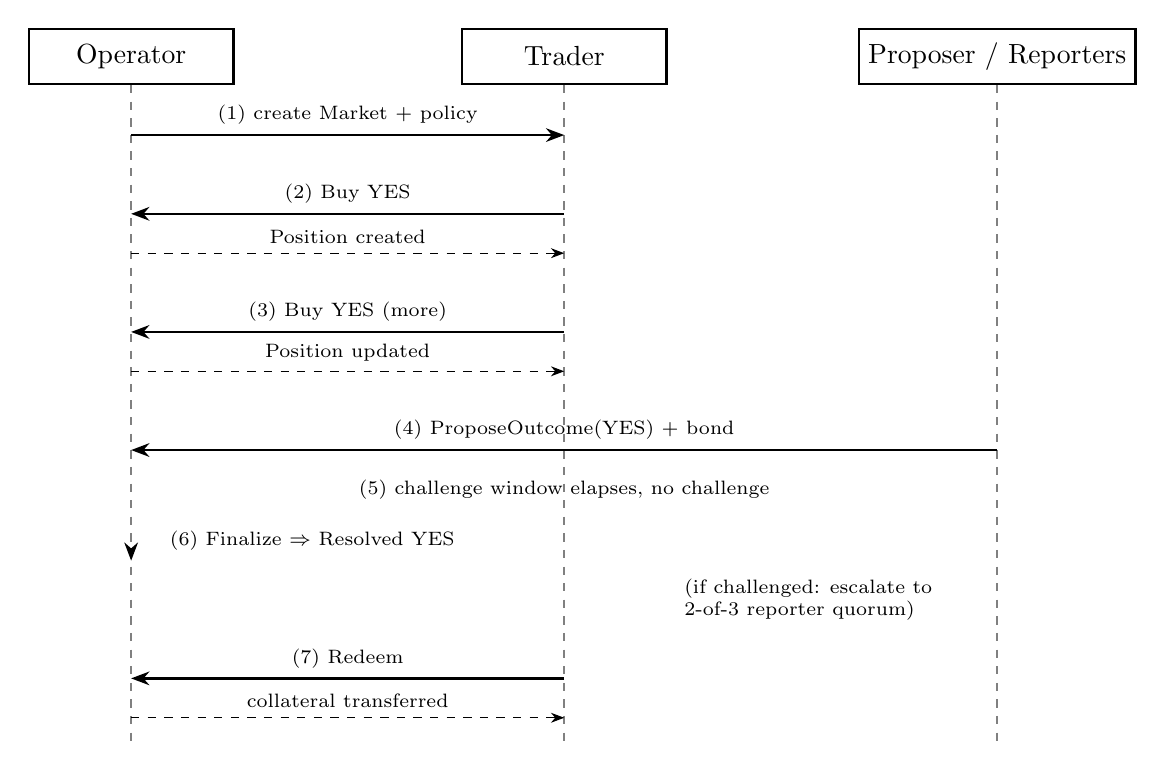
\begin{tikzpicture}[
  lifeline/.style={thick, dashed, gray},
  msg/.style={->, >=Stealth, thick},
  ret/.style={->, >=Stealth, thin, dashed},
  box/.style={draw, thick, minimum width=2.6cm, minimum height=0.7cm, fill=white}
]
\node[box] (op) at (0,0)  {Operator};
\node[box] (tr) at (5.5,0) {Trader};
\node[box] (rs) at (11,0)  {Proposer / Reporters};

\draw[lifeline] (op.south) -- (0,-8.7);
\draw[lifeline] (tr.south) -- (5.5,-8.7);
\draw[lifeline] (rs.south) -- (11,-8.7);

\draw[msg] (0,-1)   -- node[above, font=\scriptsize]{(1) create Market + policy} (5.5,-1);
\draw[msg] (5.5,-2) -- node[above, font=\scriptsize]{(2) Buy YES} (0,-2);
\draw[ret] (0,-2.5) -- node[above, font=\scriptsize]{Position created} (5.5,-2.5);
\draw[msg] (5.5,-3.5) -- node[above, font=\scriptsize]{(3) Buy YES (more)} (0,-3.5);
\draw[ret] (0,-4)   -- node[above, font=\scriptsize]{Position updated} (5.5,-4);
\draw[msg] (11,-5)  -- node[above, font=\scriptsize]{(4) ProposeOutcome(YES) + bond} (0,-5);
\node[font=\scriptsize] at (5.5,-5.5) {(5) challenge window elapses, no challenge};
\draw[msg] (0,-6.3) -- ([yshift=-3pt]0,-6.3);
\node[font=\scriptsize] at (2.3,-6.15) {(6) Finalize $\Rightarrow$ Resolved YES};
\node[font=\scriptsize, align=left] at (8.6,-6.9) {(if challenged: escalate to\\ 2-of-3 reporter quorum)};
\draw[msg] (5.5,-7.9) -- node[above, font=\scriptsize]{(7) Redeem} (0,-7.9);
\draw[ret] (0,-8.4) -- node[above, font=\scriptsize]{collateral transferred} (5.5,-8.4);
\end{tikzpicture}
\caption{Lifecycle with the optimistic tier (T3) over a reporter-quorum backstop (T2). Happy path: a single bonded proposal finalizes after an unchallenged window. On challenge, resolution escalates objectively to the quorum, never to a vote.}
\end{figure}

\begin{sloppypar}
\begin{enumerate}[leftmargin=2em, itemsep=3pt]
\item The operator creates the \texttt{Market} with a Resolution Policy: Opta's endpoint in \texttt{sources}, three reporter parties with \texttt{quorum = 2}, a 6-hour \texttt{challengeSecs}, a bond, an expiry on the match date, and a 24-hour grace period.
\item A trader exercises \texttt{Buy} for 50 YES shares with a max price of 0.55; the pm-AMM quotes, retains the fee, and creates a Position. YES reserve falls; the marginal YES price rises.
\item A second \texttt{Buy} moves the price further; each trade is an independent Daml transaction.
\item After the match, a proposer (which may be the operator, a reporter, or any allowlisted party) reads Opta and exercises \texttt{ProposeOutcome(YES)} with a bond. The Market enters \texttt{Proposed YES}.
\item The 6-hour challenge window elapses with no challenge --- the result is uncontroversial.
\item Anyone exercises \texttt{Finalize}; the Market transitions to \texttt{Resolved YES} and the proposer's bond is returned. (Had a challenger bonded the opposite, \texttt{Finalize} would first gather the 2-of-3 reporter attestations, settle to their agreed outcome, and slash the losing party's bond to the winner.)
\item Trader exercises \texttt{Redeem} on each YES Position; one collateral unit per winning share transfers from the treasury, and the Position is archived.
\end{enumerate}
\end{sloppypar}

% ---- PREDICTION MODEL MARKETPLACE ----
\section{Prediction Model Marketplace}
\label{sec:models}

The engagement deficit of \S2 is the gap between the people who \emph{know} and the people who \emph{trade}. TruthOracle closes it with an optional marketplace in which forecasters commit timestamped predictions on-ledger and are paid from a fee-funded prize pool when they outperform the market --- the ``beat the model'' loop. Models run wherever their authors like; only their \emph{outputs} --- timestamped forecasts --- are posted to Canton, so a forecaster's intellectual property never leaves their own infrastructure. The ledger's append-only ordering provides the one property scoring needs: a forecast was committed \emph{before} the outcome was known.

\subsection{Concept}

A forecaster (a data scientist, a quant desk, or an AI agent) registers a model and publishes, for each open market, a probability forecast $q \in [0,1]$ for the YES outcome. The platform aggregates a curated subset of models into a reference forecast, ``\emph{The Model},'' published alongside the pm-AMM price. Traders ``beat the model'' by trading against it; forecasters ``beat the market'' by being better calibrated than the pm-AMM price at the same instant. After resolution (\S\ref{sec:resolution}), every committed forecast is scored against the realised outcome with a proper scoring rule and a prize pool funded by a slice of trading fees is distributed in proportion to accuracy --- a Kaggle / OnlyDust competition settled trustlessly on-ledger.

\subsection{Contracts and how they are achieved in Daml}

\begin{center}
\begin{tabular}{p{3.6cm} p{10.4cm}}
\toprule
\textbf{Contract} & \textbf{Role} \\
\midrule
Prediction Model & Registry entry signed by the model author: model id, description, payout party. \\
Model Forecast & An immutable, timestamped forecast $q \in [0,1]$ for a specific Market, signed by the author; creatable only while the Market is \texttt{Trading}. \\
Model Prize Pool & A pool, signed by operator and treasury, funded by a configured fraction of \texttt{feeBps} on every trade; references its Market. \\
\bottomrule
\end{tabular}
\end{center}

\begin{enumerate}[leftmargin=2em, itemsep=3pt]
\item \textbf{Commitment before outcome.} A \texttt{ModelForecast} can be created only while the Market is \texttt{Trading} (\texttt{now < expiry}). Because Canton transactions are ordered and immutable, the recorded timestamp is unforgeable proof-of-priority: the author could not have seen the resolved outcome when committing. The ledger establishes \emph{when} a forecast was fixed, which is all a fair scoring competition requires; \emph{how} the forecast was computed is the author's private concern.
\item \textbf{Funding the pool.} Each \texttt{Buy}/\texttt{Sell} routes a configured fraction of its fee into the Market's \texttt{ModelPrizePool} atomically with the trade, so the pool balance is a deterministic function of volume.
\item \textbf{Scoring.} On resolution a \texttt{ScoreAndDistribute} choice reads every \texttt{ModelForecast} and computes each model's Brier score $s = (q - o)^2$ against the realised $o \in \{0,1\}$ (lower is better; log score is an alternative). Scoring is pure Daml arithmetic over committed values --- deterministic and independently reproducible by any audit observer.
\item \textbf{Distribution.} The pool is split in inverse proportion to score (weight $w_i = 1 - s_i$, payout $= \text{pool}\cdot w_i / \sum_j w_j$), optionally gated so only models that beat the pm-AMM-implied probability at their forecast's timestamp are paid. Payouts are collateral transfers to each author's payout party.
\item \textbf{``The Model''.} The reference forecast is a deterministic aggregation (e.g., the accuracy-weighted mean of a curated subset of forecasts) recomputed and published by the operator; it carries no special on-ledger authority beyond being the number traders choose to trade against.
\end{enumerate}

\subsection{Social and agent layer}

Forecasts, ``The Model,'' and resolved outcomes are surfaced through an off-ledger product layer --- bots and LLM agents that post to Telegram and X, reply to users, and turn forecasts into shareable graphics. This layer reads and writes the public projection of market state, carries no protocol authority, and is out of scope for the on-ledger specification, but it is how the marketplace captures the non-trading expert audience of \S2.

% ---- RATIONALE ----
\section{Rationale}

\subsection{Core Thesis}

Prediction markets are a primitive financial instrument; their slow adoption is structural, not demand-driven. Thin liquidity, slow and contested resolution, and limited regulatory accommodation have confined them to short-lived high-attention events. Canton addresses the regulatory problem, pm-AMM the liquidity problem, and tiered objective resolution the contestation problem. With those constraints lifted, prediction markets generalise from a niche to a class of contracts comparable to options or futures in scope.

\subsection{Design Decisions}
\label{sec:design}

\begin{enumerate}[leftmargin=2em, itemsep=3pt]
\item \textbf{Provenance from signatures and authorization.} Sources and reporters are named, accountable, allowlisted parties, so a signature --- enforced by Daml's authorization model --- is sufficient to establish where a value came from. Resolution is built directly on this: ordinary \texttt{sha256} commitments and \texttt{secp256k1} signature checks, and nothing heavier to deploy or operate.
\item \textbf{Objective tiers, never intersubjective voting.} Every tier resolves to ``what an authoritative source reported'' (Kalshi/Chainlink/Pyth), not ``what a token quorum decided'' (UMA/Augur). A licensed venue cannot accept the latter; the pitch's ``objectively resolvable answer from specified sources'' demands the former.
\item \textbf{Optimism for UX, objectivity for truth.} T3 keeps Polymarket's open, fast, bonded propose-and-challenge flow but escalates disputes to T1/T2 rather than to a vote --- speed and openness without intersubjectivity.
\item \textbf{First-party signing as the ideal.} Where a source can sign (T1), trust collapses to the source's own key with no intermediary to vouch for the data --- the strongest provenance the protocol can offer, and the preferred tier wherever a source supports it.
\item \textbf{Reserves on the Market, not a separate Pool.} Folding pm-AMM reserves into the Market removes a dereferencing step and a class of authorization errors, at the cost of the same per-market trade serialisation an external Pool would impose.
\item \textbf{Positions signed by the trader.} The operator is an observer for accounting but cannot modify or archive a Position; regulators obtain position data through audit observers, not operator key custody.
\item \textbf{Void as a first-class outcome.} Abandoned matches, overturned elections, dead APIs, and unresolvable disputes settle honestly to \texttt{Void} (cost basis returned) rather than forcing a bad-faith YES/NO.
\item \textbf{Policy immutable after creation.} Sources, source keys, reporters, quorum, challenge window, and bond are all fixed at creation, so an operator cannot retroactively choose a favourable source or captive reporter; audit observers see the full policy ex ante.
\item \textbf{Model outputs on-ledger, models off-ledger.} The marketplace commits forecast outputs only; ledger ordering establishes that a forecast preceded the outcome, which is all scoring needs, while each forecaster's model and data stay on their own infrastructure.
\end{enumerate}

% ---- SECURITY ----
\section{Risk and Security Considerations}

\textbf{Source and reporter allowlist integrity.} The protocol is only as honest as the sources, source keys, and reporters named at creation. Mitigations: include at least one audit observer independent of the operator; for production markets require T2 quorum across reporters operated by distinct entities, and prefer T1 first-party signing where available.

\textbf{Reporter / proposer collusion.} A colluding T2 quorum, or a coordinated T3 proposer and challenger, can settle dishonestly. The quorum size, reporter diversity, and bond size are the defences; all are immutable and audit-visible. Reporters and proposers are licensed parties subject to off-ledger legal accountability that anonymous public-chain oracles lack.

\textbf{Source compromise (residual).} A compromised source can serve a forged response that signs validly (T1) or that every reporter reads faithfully (T2), yielding a wrong resolution. This residual risk is inherent to any objective oracle and is mitigated by source diversity, the T3 challenge path, the audit-observer dispute path, and the \texttt{Void} fallback.

\textbf{Signature-scheme and key-rotation hygiene (T1).} On-ledger \texttt{secp256k1} verification is only as good as the pinned key. Keys are pinned at creation and immutable; sources must coordinate rotation under controlled change-management, and a rotated-away key simply fails verification (failing safe) rather than silently accepting.

\textbf{pm-AMM manipulation.} A well-capitalised trader can move the price before resolution, but pays for the impact and absorbs the reversion loss; \texttt{feeBps} should make round-trip manipulation unprofitable.

\textbf{Resolution / challenge timing.} The grace period bounds how long a market stays unresolved; the challenge window trades speed against dispute opportunity. Set per category: short windows and 24-hour grace for finalised sports, longer for electoral or litigation-resolvable markets.

\textbf{Prize-pool gaming.} Forecast spam or sockpuppet models can dilute honest payouts. Mitigations: cap forecasts per author per market, charge a registration stake for a \texttt{PredictionModel}, and gate payouts behind a beat-the-market threshold.

\textbf{Privacy under audit observation.} Audit observers see all Positions under their Market. The audit-observer field is mutable only via a Market-level choice controlled by operator and treasury jointly, so accidental disclosure cannot occur from a unilateral key.

\textbf{Front-running.} Transaction ordering is the synchronization domain's sequencer; the protocol does not defend against a malicious sequencer. Licensed operators should select a domain whose sequencer governance their regulator accepts.

\textbf{Collateral token risks.} The Market accepts any CIP-56-compliant token; restricting \texttt{collateralToken} to regulated stablecoins or Canton Coin per jurisdiction is an operator policy.

% ---- BACKWARDS COMPATIBILITY ----
\section{Backwards Compatibility}

This proposal introduces new Daml template definitions only and requires no changes to existing Daml models, the Canton protocol, or synchronization domain software. It is fully backwards compatible at the protocol layer. The only external dependency is CIP-56 (token semantics for collateral); the cryptographic primitives used (\texttt{sha256}, \texttt{secp256k1}) ship in the Daml standard library (\texttt{DA.Crypto.Text}) and require no additional packages. Successor versions are published by bumping the \texttt{version:} field in \texttt{daml.yaml} while keeping the package \texttt{name:} stable, so Canton's package upgrade semantics recognise them as in-place upgrades.

% ---- REFERENCE IMPLEMENTATION ----
\section{Reference Implementation}
\label{sec:refimpl}

A reference implementation, including a Daml Script test suite, lives in the Cantor8 monorepo at \texttt{daml/TruthOracle/} and targets Daml SDK 3.x. The suite passes against both the in-memory IDE ledger and the persistent Canton sandbox, covering pm-AMM invariants, all four resolution tiers (T1 signature verification, T2 quorum agreement and disagreement, T3 unchallenged finalize and challenged escalation), expired-without-resolution voiding, and prize-pool scoring. It is released under Apache-2.0 and currently deployed on Canton DevNet at the operator party \texttt{TruthOracle::devnet}.

The DAR is released under a stable package \texttt{name}; new versions are published by bumping the \texttt{version:} field in \texttt{daml.yaml} while keeping the package \texttt{name:} stable, as required for Canton's package upgrade semantics to recognise successor packages as in-place upgrades.

% ---- ROLLOUT ----
\section{Implementation and Rollout}

\noindent\textbf{Phase 1 --- Daml Templates and Local Testing.} Reference implementation of \texttt{Market}, \texttt{Position}, \texttt{LiquidityPosition}, and \texttt{OutcomeAttestation}, with Daml Script tests covering pm-AMM invariants and all four resolution tiers and their edge cases. Submitted as a pull request to the Cantor8 protocol-extensions repository. No on-chain governance action required.

\smallskip
\noindent\textbf{Phase 2 --- DevNet Pilot.} Operator party \texttt{TruthOracle::devnet} deploys with three pilot markets: one T0, one T2 (2-of-3 reporters), one T3-over-T2. Cantor8 enterprise-wallet users are invited. Success criteria: $\geq$ 90 distinct trader parties, $\geq$ 500 \texttt{Buy} transactions, zero failed-resolution incidents, and pm-AMM invariant integrity verified by an independent audit observer.

\smallskip
\noindent\textbf{Phase 3 --- Licensed MainNet Launch.} Following operator licensing (Belarus, then Korea), the DAR is deployed on the Global Synchronizer under the licensed operator party, with reporters operated by distinct accountable entities and T1 signing onboarded with at least one signed data feed. Initial scope: sports events resolved against Opta. KYC-gated observability is enforced through party allocation.

\smallskip
\noindent\textbf{Phase 4 --- Prediction Model Marketplace.} The \texttt{PredictionModel}, \texttt{ModelForecast}, and \texttt{ModelPrizePool} contracts of \S\ref{sec:models} are deployed, letting data scientists and AI agents submit forecasts and earn from a fee-funded prize pool, with the social/agent layer surfacing ``The Model'' and outcomes to a non-trading expert audience.

\smallskip
\noindent\textbf{Dependencies.} CIP-56 (token semantics for collateral). No changes to the Canton protocol or synchronization domain software; the entire proposal is implementable at the Daml application layer, with no proving or verifying infrastructure of any kind.

\bigskip
\noindent\textbf{Changelog}

\smallskip
\textit{v0.7 (22 July 2026).} Aligns the specification with the reference pm-AMM execution model: adds the \emph{complete-set} primitives \texttt{Split}/\texttt{Merge} (one collateral unit $\leftrightarrow$ one YES + one NO) as the sole collateral on/off ramp, the direct outcome-token swap \texttt{SwapShares} with \texttt{Buy}/\texttt{Sell} specified as mint-and-swap composites, the cached-price / virtual-reserve execution model (trades run against closed-form optimal reserves at the cached price; physical reserves custody inventory), and the optional pre-trading \emph{liquidity period} for dynamic pools (swaps disabled, liquidity and minting open; the decay anchor for $L_{\mathrm{eff}}$).

\smallskip
\textit{v0.6 (27 June 2026).} Adopts Paradigm's \textbf{dynamic pm-AMM} (Gaussian score dynamics) in place of the constant-product curve: marginal price $P=\Phi((y-x)/L_{\mathrm{eff}})$ with time-decaying $L_{\mathrm{eff}}=L\sqrt{T-t}$, value-based liquidity provision, and uniform loss-versus-rebalancing for LPs, backed by a Daml normal-distribution and invariant-solver math library. Adds the off-ledger \textbf{read model} (Participant Query Store) powering dashboards and audit position-book reporting, and the \textbf{operator console and key management} control plane (market creation, \texttt{ResolutionPolicy} authoring, audit-observer administration, and source/reporter signing-key custody and rotation). Retains the four-tier objective resolution model, the Canton privacy model, and the optional Prediction Model marketplace.

\smallskip
\textit{v0.5 (10 June 2026).} Consolidated specification. Defines the four-tier objective resolution model --- T0 designated operator (Kalshi), T1 first-party signed source verified on-ledger with \texttt{secp256k1} (Pyth / API3), T2 independent reporter quorum (Chainlink), and T3 optimistic propose-and-challenge with objective escalation (Polymarket UX, no token voting) --- together with the \texttt{ResolutionPolicy} record and the \texttt{OutcomeAttestation} contract. Adds a survey of how existing prediction markets resolve. Retains the constant-function pm-AMM, the Canton privacy model, and the Prediction Model marketplace.

\smallskip
\textit{v0.4 (10 June 2026).} Introduced an $M$-of-$N$ quorum of signed attestations from designated resolver parties; promoted the Prediction Model marketplace to a specified section.

\smallskip
\textit{v0.3 (28 May 2026).} Working draft establishing the four-template Daml protocol, the pm-AMM pricing model, the four-phase market lifecycle, the rationale, the risk model, and the rollout plan.

\bigskip
\noindent\textbf{References}

\smallskip
\noindent Paradigm, \emph{pm-AMM} (November 2024). \url{https://www.paradigm.xyz/2024/11/pm-amm}

\bigskip
\noindent\textbf{Copyright}

This proposal is licensed under the Apache License, Version 2.0.

\end{document}
